% kapitel5.tex
\externaldocument{C_anhang.tex}
\chapter{Evaluation}
\label{chapter:evaluation}

\section{Versuchsaufbau}
\label{section:versuchsaufbau}
Im Folgenden werden der Versuchsaufbau und die Versuchsdurchführung beschrieben.

\subsection{Komponenten}

\paragraph{Eyetracking}
Die Komponenten des Eyetracking werden in \acs{abb}~\ref{fig:komponenten} gezeigt. Der stimuluspräsentierende Bildschirm ist über einen eigenen PC mit der Workstation verbunden. Die Workstation ist mit der \acs{et} konnektiert und führt die \iV Software aus. 

\begin{figure}[ht]
\begin{center}
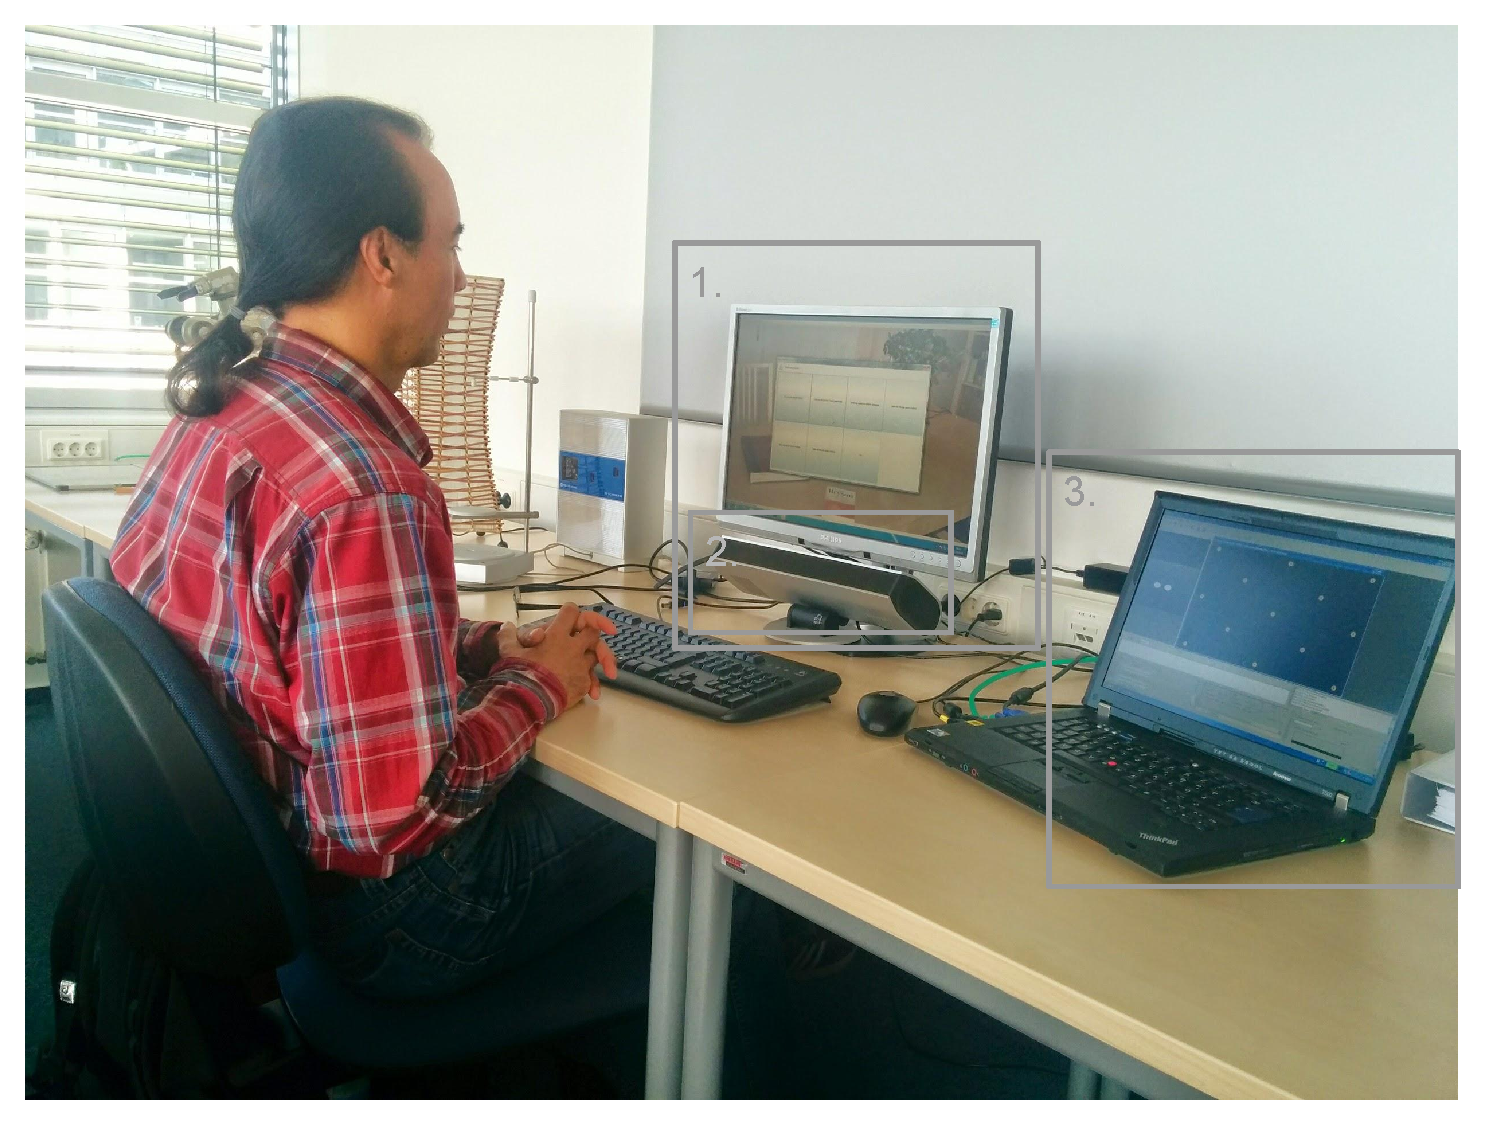
\includegraphics[width=0.7\textwidth]{bilder/evaluation/anordung.pdf}\hfill
\end{center}
\caption{Komponenten des Eyetracking. Die Darstellung zeigt eine Testperson während der Verwendung des Softwareprototyp von Eidam (2015). Dieser Aufbau wurde für die vorliegende Arbeit übernommen.  (1.)~\acs{spb}, (2.)~\acs{et}, (3.)~\iV ~\acs{wo}. (Bild:~modifiziert aus \cite[S.51]{Eidam2015})}
\label{fig:komponenten}
\end{figure}

Bei der Versuchsdurchführung ist auf eine adäquate Sitzpositionierung der Testperson im Verhältnis zum Bildschirm zu achten. Die Augen der Testperson sollten von einer tiefer angeordneten Position der RED observiert werden, \vgl~\acs{abb}~\ref{fig:empfehlung}. Grundsätzlich soll ein freies Sichtfeld gewährleistet sein.

\paragraph{\acf{tps}}
Der als Telepräsenzsystem modifizierte Roomba 620 wird in \acs{abb} \ref{fig:subroomba} dargestellt. Zu erkennen ist die zentrisch angeordnete Kamera der Firma Axis (AXIS M1034-W) und der Access-Point, der an der seriellen Schnittstelle des Roombas angeschlossen ist. Der Access-Point dient unter Zuhilfenahme von \enquote{socat}-Prozessen dazu, die Netzwerkkommunikation zu ermöglichen. \enquote{Socat} ist ein Tool, um Datenströme unter Linux/Unix-Systemen verbinden zu können. Für die vorliegende Arbeite wurde \enquote{socat} so konfiguriert, dass es an einem Netzwerk-Socket (einem TCP-Port) lauscht und die Daten der TCP-Pakete an den seriellen Port weiter leitet. Im Gegenzug werden die Daten aus der seriellen Schnittstelle an die zuletzt geöffnete TCP-Verbindung zurückgeliefert. %Auf die Nutzung dieser zweiten genannten Verbindungsrichtung wurde im Rahmen der vorliegende Arbeit verzichtet.
 
\begin{figure}[ht]
\begin{minipage}[b]{\linewidth} 
      \centering 
  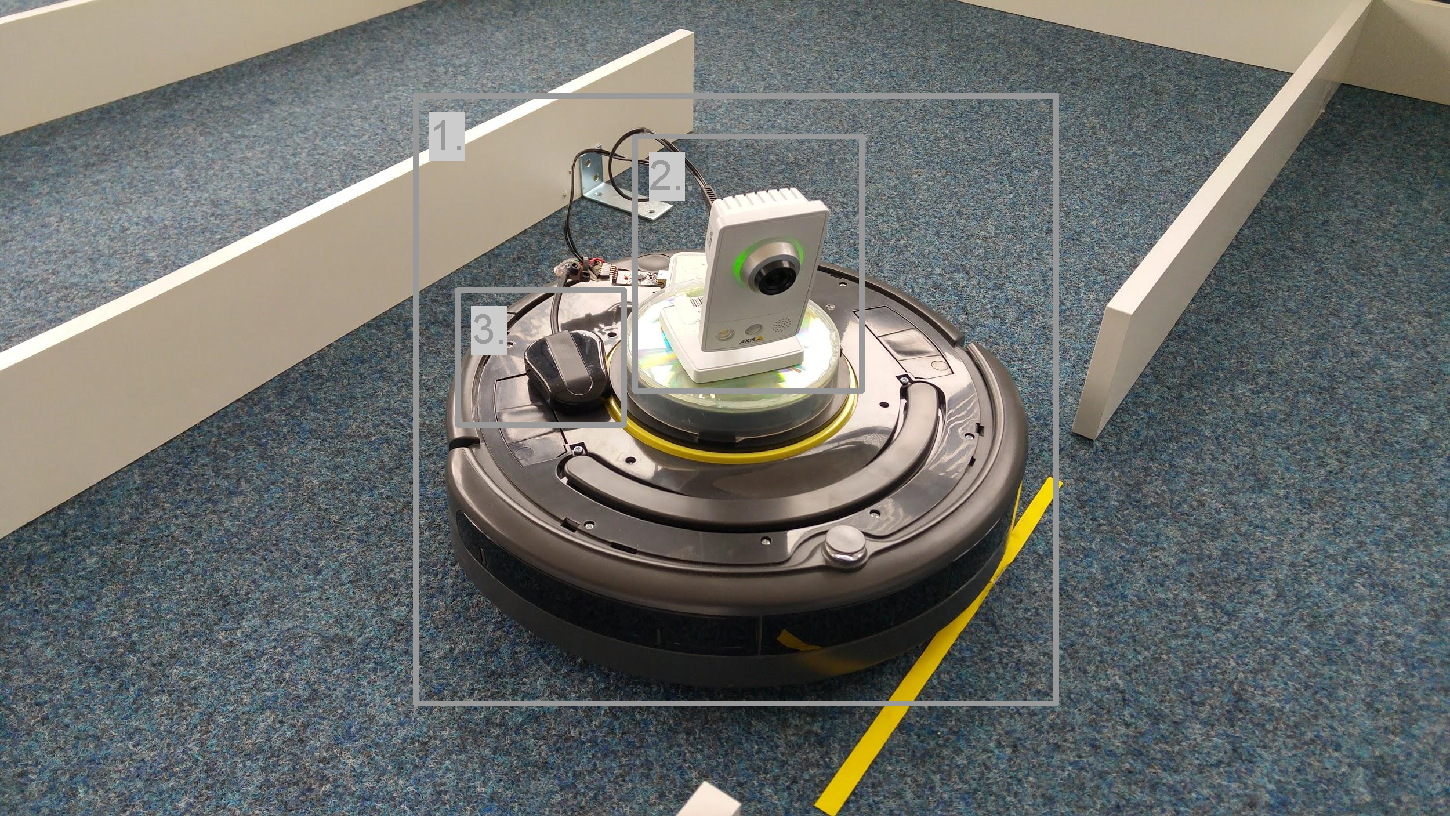
\includegraphics[width=0.7\linewidth]{bilder/evaluation/roomba.pdf}
  \label{fig:subroomba} 
   \end{minipage}%
\caption{Verwendetes \acl{tps} während der Parcoursdurchquerung. (1.)~Roomba 620 modifiziert als \acl{tps}, (2.)~mittig angeordnete Videokamera, (3.)~Access-Point zur Netzwerkkommunikation.}
\label{fig:subroomba}
\end{figure}


\subsection{Testpersonen}
Für die Durchführung der Parcoursaufgabe und der Evaluation des Fragebogens stellten sich insgesamt fünf körperlich unbeeinträchtigte Testpersonen zu Verfügung. Vier Personen aus dem Lehrgebiet der Mensch-Computer-Interaktion des Fachbereichs Mathematik und Informatik der FernUniversität Hagen nahmen freiwillig daran teil. Ferner beteiligte sich der Verfasser dieser Arbeit ebenfalls an Evaluation und Parcoursaufgabe. In Bezug auf die Nutzung von Eyetracking-Systemen unterschieden sich die Teilnehmer in ihren Vorerfahrung, die aber nicht weiter differenziert oder unterschieden wurde. Jede Testperson bekam vor der Kalibrierung des Eyetracking-Systems eine kurze Einführung in die grundlegenden Funktionsweisen der beiden Steuerungsmodi und war im Anschluss angehalten, nach eigenem Ermessen die Parcoursbewältigungsaufgabe durchzuführen.

\subsection{Testparcours}
Der eigentliche Testparcours befindet sich innerhalb eines Bereichs der Größe 200 cm x 200 cm. Hierbei wird der Bereich durch einen 80 cm x 80 cm großen Ladestationsbereich erweitert. Der Zugang zum eigentlichen Parcours ist durch eine Eingangsbarriere der Größe von 40 cm festgelegt. Innerhalb dieses Abschnittes ist eine Art \enquote{Kreisbahn} durch eine 50 cm breite \enquote{Strecke} eingerichtet, siehe \acs{abb}~\ref{fig:aufbau}.

\begin{figure}[ht]
\begin{center}
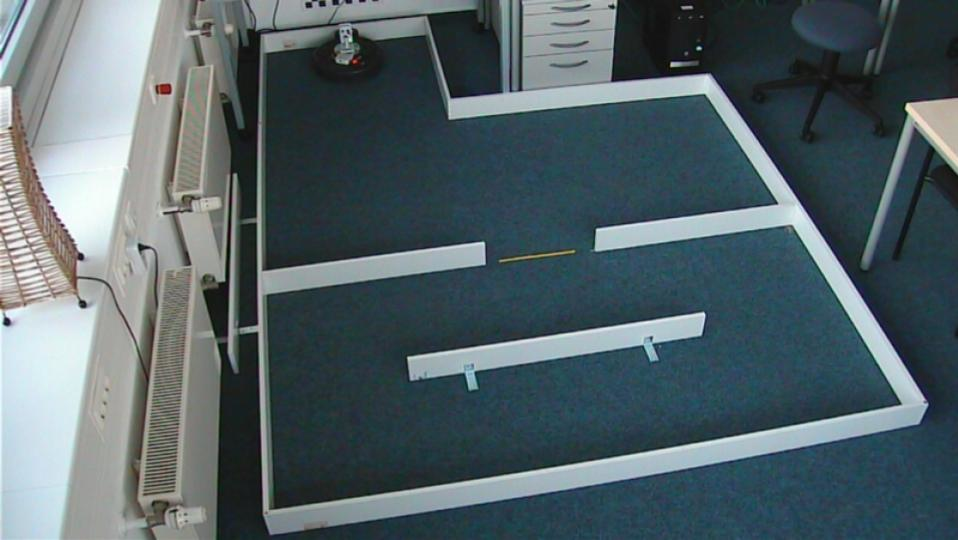
\includegraphics[width=0.7\textwidth]{bilder/evaluation/TopView.png}\hfill
%\includegraphics[scale=0.2]{bilder/evaluation/Parcour.png}
\end{center}
\caption{Parcours-Versuchsaufbau mit einer Ansicht von oben. Zu erkennen ist der eigentliche Testparcours. Start und Stopp sind anhand der gelben Markierung in der Eingangsbarriere auszumachen.}
\label{fig:aufbau}
\end{figure}


\section{Versuchsdurchführung}
\label{section:versuchsdurchführung}
Die folgenden Systemeinstellungen wurden von allen beteiligten Testpersonen verwendet. Die Einstellungen kamen für beide Steuermethoden zum Einsatz. Prinzipiell konnten die Einstellungen frei gewählt werden. Alle Benutzer entschieden sich jedoch für die Standardeinstellung:

\begin{itemize}
 \item[-] 1000 ms Fixierungsdauer,
 \item[-] 250 ms minimale Lidschlussdauer und 500 ms maximale Lidschlussdauer,
 \item[-] 200 px maximale Dispersion,
 \item[-] 200 px maximale Auslenkung in Bezug auf die horizontale und vertikale Augengestenerkennung.
\end{itemize}

Zur Messung der Steuerung wurde ein Parcoursaufgabe konzipiert, wobei die zurückgelegte Zeit als quantitatives Messkriterium herangezogen wurde. Ziel dieser Anordnung war es, die Aufgabe in einer möglichst kurzen Zeit zu bewältigen. Die Vermeidung von Kollisionen war beabsichtigt, jedoch kein Abbruchkriterium. Die Aufgabe galt als erfolgreich beendet, wenn der Parcours ausgehend von der Startmarkierung einmal umfahren und anschließend die Markierung überquert wurde. Die Richtung der Durchführung blieb den Testpersonen überlassen und wurde nicht unterschieden.

Nach Abschluss der Parcoursaufgabe wurde zur Klärung der Gebrauchstauglichkeit (Usability) des Prototyps ein eigens konzipierter Fragebogen mit den in Kapitel~\ref{sect:testmerkmale} Testmerkmalen beantwortet, \vgl Anhang~\ref{chapter:ergabb}. 

